% !TEX root = main.tex

\section{Path explosion}
\label{se:path-explosion}

One of the main challenges of symbolic execution is the path explosion problem: a symbolic executor may fork off a new state at every branch of the program, and the total number of states may easily become exponential in the number of branches. Keeping track of a large number of pending branches to be explored, in turn, impacts both the running time and the space requirements of the symbolic executor. 

The main sources of path explosion are loops and function calls. Each iteration of a loop can be seen as an {\tt if-goto} statement, leading to a conditional branch in the execution tree. If the loop condition involves one or more symbolic values, the number of generated branches may be potentially infinite, as suggested by the following example. 

\begin{figure}[t]
\begin{center}
\begin{tabular}{c}
\begin{lstlisting}[basicstyle=\ttfamily\scriptsize]
1.  int x = sym_input(); // e.g., read from file
2.  while (x > 0) {
3.     x = sym_input();  
4.  }
\end{lstlisting}
\end{tabular}
\end{center}
\vspace{-2mm}
\caption{Loop example with input read from the environment~\protect\cite{CS-CACM13}.}
\label{fi:example-loop}
\end{figure}

\vspace{-2pt} % TODO
\boxedexample{Consider the code fragment of Figure~\ref{fi:example-loop}~\cite{CS-CACM13}, where \texttt{sym\_input()} is an external routine that interacts with the environment (e.g., by reading input data from a network) and returns a fresh symbolic input. The path constraint set at any final state has the form: 
\[ \pi = \left ( \bigwedge_{i \in [1, k]} \alpha_i > 0 \right ) \wedge (\alpha_{k+1} \leq 0) \] 
where $k$ is the number of iterations and $\alpha_i$ is the symbol produced by \texttt{sym\_input()} at the $i$-th iteration.}

While it would be simple (and is indeed common) to bound the loop exploration up to a limited number of iterations, interesting paths could be easily missed with this approach.  A large number of works have thus explored more advanced strategies, e.g., by characterizing similarities across distinct loop iterations or function invocations through summarization strategies that prevent repeated explorations of a code portion or by inferring invariants that inductively describe the properties of a computation. In the remainder of this section we present a variety of prominent techniques, often based on the computation of an under-approximation of the analysis with the aim of exploring only a relevant subset of the state space.

% ---------------------------------------------------------------------------------------------------
\subsection{Pruning Unrealizable Paths}
\label{ss:unrealizable-paths}

A first natural strategy to reduce the path space is to invoke the constraint solver at each branch, pruning unrealizable branches: if the solver can prove that the logical formula given by the path constraints of a branch is not satisfiable, then no assignment of the program input values could drive a real execution towards that path, which can be safely discarded by the symbolic engine without affecting soundness. \mytempedit{An example of this strategy is provided in Figure~\ref{fig:eager-evaluation}.}

\iffullver{
\boxedexample{Consider the example shown in Figure~\ref{fig:eager-evaluation} and assume that {\tt a} is a local variable bound to an unconstrained symbol $\alpha_a$. A symbolic engine would start the execution of the code fragment of Figure~\ref{fig:eager-evaluation}a by evaluating the branch condition $a > 0$. Before expanding both branches, the symbolic engine queries a constraint solver to verify that no contradiction arises when adding to the path constraints $\pi$ the {\em true} branch condition ($\alpha_a > 0$) or the {\em false} branch condition ($\alpha_a \leq 0$). Since both paths are feasible, the engine forks the execution states B and D (see Figure~\ref{fig:eager-evaluation}b). A similar scenario happens when the engine evaluates the branch condition $a > 1$. However, since $\alpha_a$ is not unconstrained anymore, some contradictions are actually possible. The engine queries the solver to check the following path constraints: (1) $\alpha_a > 0~\wedge~\alpha_a > 1$, (2)~$\alpha_a > 0~\wedge~\alpha_a \leq 1$, (3) $\alpha_a \leq 0~\wedge~\alpha_a > 1$, and (4) $\alpha_a \leq 0~\wedge~\alpha_a \leq 1$. The formula $\alpha_a \leq 0 \wedge \alpha_a > 1$, however, does not admit a valid solution and therefore the related path can be safely dropped by the engine. %On the other hand, other paths admit a valid solution and can be further explored by the engine.
}
}

\begin{figure}[t]
  %\vspace{-3mm}
  %\centering
  \begin{subfigure}{.29\textwidth}
    \vspace{0mm}
    \begin{lstlisting}[basicstyle=\ttfamily\scriptsize]
   if (a > 0) {
      ...
   } 

   if (a > 1) {
      ...
   }
    \end{lstlisting}
    \vspace{-0.7mm}
    \caption{}
  \end{subfigure}%
  %\hspace{-2mm}
  \begin{subfigure}{.70\textwidth}
    \centering
    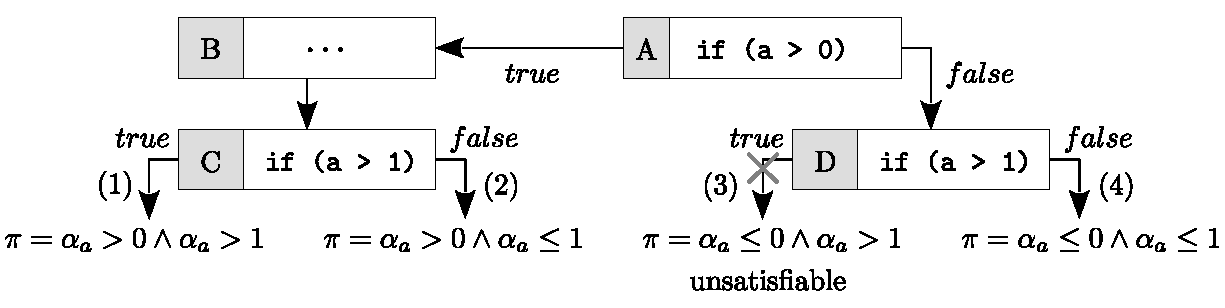
\includegraphics[width=1.0\columnwidth]{images/eager-evaluation} 
    %\label{fig:sub1}
    \vspace{-5mm}
    \caption{}
  \end{subfigure}%
  \vspace{-2mm}
  \caption{Pruning unrealizable paths example: (a) Code fragment; (b) symbolic execution of the code fragment: the {\em true} branch at node D is not explored since its path constraints $(\alpha_a \leq 0 \wedge \alpha_a > 1)$ are not satisfiable.}
  \label{fig:eager-evaluation}
\end{figure}

This approach is commonly referred to as {\em eager evaluation} of path constraints, since constraints are eagerly checked at each branch, and is typically the default in most symbolic engines. We refer to Section~\ref{se:constraint-solving} for a discussion of the opposite strategy, called {\em lazy evaluation}, aimed at reducing the burden on the constraint solver.

\mytempedit{
% This can can be seen as a set of learned conflicts and 
An orthogonal approach that can help reduce the number of paths to check is presented in~\cite{SSJ-NFM15}. While a SMT solver can be used to explore a large search space one path at a time, it will often end up reasoning over control flows shared by many paths. This work exploits this observation by extracting a minimal {\em unsat core} from each path that is proved to be unsatisfiable,
removing as many statements as possible while preserving unsatisfiability. An engine could thus exploit unsat cores to discard paths that share the same (unsatisfiable) statements.
}

\subsection{Function and Loop Summarization} 
\label{ss:summarization}

When a code fragment -- be it a function or a loop body --  is traversed several times, the symbolic executor can build a summary of its execution for subsequent reuse.

\mytempedit{\myparagraph{Function summaries}}
A function $f$ may be called multiple times throughout the execution, either at the same calling context or at different ones. Differently from plain executors, which would execute $f$ symbolically at each invocation, the compositional approach proposed in~\cite{G-POPL07} dynamically generates {\em function summaries}, allowing \mynote{I: si intende function inputs?} the executor to effectively reuse prior discovered analysis results. \mytempedit{Proposed for concolic executors, the technique captures the effects of a function invocation with a formula $\phi_w$ that conjoins \mynote{I: Perche' w a pedice? Cosa indica?} constraints on the inputs, describing equivalence classes of concrete executions, with constraints observed on the output. A function summary is a propositional logic formula defined as the disjunction of $\phi_w$ formulas from distinct classes, and feasible inter-procedural paths are  modelled by composing symbolic executions of intra-procedural ones.
%
Compositional symbolic execution has been extended in~\cite{AGT-TACAS08}: summaries are generated as first-order logic formulas with uninterpreted functions, allowing the formation of incomplete summaries (i.e., capturing only a subset of the paths within a function) that can be expanded on demand during the inter-procedural analysis as more statements get covered. 
%
% skipping it for now: not self-contained
%\mytempedit{
%\cite{CFS-PLDI09} makes a step further by describing an algorithm for generalizing symbolic summaries, effectively enhancing their reuse in practice.
%}

%A similar idea has been also proposed in~\cite{BCE-TACAS08}. The main intuition is that,
\cite{BCE-TACAS08} explores a different flavor of summarization, based on the following intuition:
}
if two states differ only for some program values that are not read later, the executions generated by the two states will produce the same side effects. Side effects of a code fragment can be therefore cached and possibly reused later.

\mytempedit{\myparagraph{Loop summaries}}
Akin to function calls, partial summarizations for loops can be obtained as described in~\cite{GL-ISSTA11}. A loop summary uses pre- and post-conditions that are dynamically computed  during the symbolic execution by reasoning on the dependencies among loop conditions and symbolic variables. Caching loop summaries not only allows the symbolic engine to avoid redundant executions of the same loop in the same program state, but  makes it also possible to generalize the summary to cover different executions of the same loop under different conditions. 

\mytempedit{
Early works can generate summaries only for loops that update symbolic variables across iterations by adding a fixed amount to them. Also, they cannot handle nested loops or {\em multi-path loops}, i.e., loops with branches within their body. Proteus~\cite{XX-FSE16} is a general framework proposed for summarizing multi-path loops. It classifies loops according to the patterns of values changes in path conditions (i.e., whether an induction variable is updated) and of the interleaving of paths within the loop (i.e., whether there is a regularity). The classification leverages an extended form of control flow graph, which is then used to construct an automata that models the interleaving. The automata is traversed in a depth-first fashion and a disjunctive summarization is constructed for all the feasible traces in it, where a trace represents an execution in the loop. The classification determines if a loop can be captured either precisely or approximately (which can still be of practical relevance), or it cannot. Precise summarization of multi-path loops with irregular patterns or non-inductive updates, and more importantly summarization of nested loops remain open research problems.
}
%Recently, the latter scenario has been effectively tackled by Proteus~\cite{XX-FSE16}. %by S-Looper~\cite{XX-ISSTA15} and later 
%S-Looper targets loops that traverse \mynote{Che vuol dire attraversare una stringa?} a string, without modifying it, and that have branch conditions related to the traversed string or other loop induction variables. Proteus makes a step further by 
%
%First, it classifies loops based on the patterns of value changes, i.e., whether the loop variables are induction or non-induction, and based on the patterns of path interleaving, i.e., whether the path interleaving can be considered {\em sequential}, {\em periodic}, or {\em irregular}. The classification is done by analyzing the flowgraph of the loop. Finally, depending of the type of the loop, different strategies are used for generating a disjunctive loop summarization (DLS). Intuitively, a DLS is the union of all the trace summaries for a loop, where a trace summary is expressed as the condition needed to meet when trace is feasible, and the value of the variables after executing the trace. For instance, for loops that have only induction variables and with a periodic pattern, trace summaries are derived by exploring with a DFS strategy the path dependency automaton (PDA) of the loop. This data structure captures the execution order and path interleaving patterns of the paths. Although not all types of loops can be summarized by Proteus, it still can produce approximated loop summaries for many different types, which could be useful in practice. Precise summarization of multi-path loops with non-induction variables or with an irregular pattern, or even worse summarization of nested loops, still remain an open research problem. 

%This work proposes a general framework for summarizing multi-path loops. First, it classifies loops based on the patterns of value changes, i.e., whether the loop variables are induction or non-induction, and based on the patterns of path interleaving, i.e., whether the path interleaving can be considered {\em sequential}, {\em periodic}, or {\em irregular}. The classification is done by analyzing the flowgraph of the loop. Finally, depending of the type of the loop, different strategies are used for generating a disjunctive loop summarization (DLS). Intuitively, a DLS is the union of all the trace summaries for a loop, where a trace summary is expressed as the condition needed to meet when trace is feasible, and the value of the variables after executing the trace. For instance, for loops that have only induction variables and with a periodic pattern, trace summaries are derived by exploring with a DFS strategy the path dependency automaton (PDA) of the loop. This data structure captures the execution order and path interleaving patterns of the paths. Although not all types of loops can be summarized by Proteus, it still can produce approximated loop summaries for many different types, which could be useful in practice. Precise summarization of multi-path loops with non-induction variables or with an irregular pattern, or even worse summarization of nested loops, still remain an open research problem. 

%In order to perform loop classification, Proteus constructs a flowgraph of the sliced loop program. Loop slicing is performed exploiting the program dependence graph (PDG), which combines the control flow graph (CFG) and the data dependencies of the loop. The flowgraph is then analyzed and the loop classified. Depending of the type of the loop, different strategies are used for generating a disjunctive loop summarization (DLS). Intuitively, a DLS is the union of all the trace summaries for a loop. For instance, loops that contain only induction variables and that have a path interleaving with a periodic pattern are summarized by first constructing the path dependency automaton (PDA) of the loop, then by summarizing the effect of distinct paths (periods) of the cycle and finally by relating these effects to the execution number of the loop. Although not all types of loops can be summarized by Proteus, it still can produce approximated loop summaries for many different types, which could be useful in practice. Precise summarization of multi-path loops with non-induction variables or with an irregular pattern, or even worse summarization of nested loops, still remain an open research problem. 

Of a different flavor is the compaction technique introduced in~\cite{SST-ATVA13}, where \mynote{I: Ha senso qui? Altrimenti dove?} the analysis of cyclic paths in the control flow graph yields {\em templates} that declaratively describe the program states generated by a portion of code \myedit{as} a \myedit{\em compact} symbolic execution tree. By exploiting templates, the symbolic execution engine can explore a significantly reduced number of program states. A drawback of this approach is that templates introduce quantifiers in the path constraints: in turn, this may significantly increase the burden on the constraint solver.

% ---------------------------------------------------------------------------------------------------
\subsection{Interpolation} 
\label{ss:interpolation}
\mytempedit{
Modern SAT solvers rely on a mutual reinforcing combination of search and deduction, using the latter to drive the former away from a conflict when it becomes blocked. In a similar manner, symbolic execution can benefit from {\em interpolation} techniques to derive properties from program paths that did not show a desired property, so to prevent the execution from exploring other paths that would lead to a failure in the same way.

{\em Craig interpolants}~\cite{Craig1957} allow deciding what information about a formula is relevant to a property. Assuming a formula $P\rightarrow Q$ holds in some logic, it is possible to construct an interpolant $I$ such \mynote{I: ma la freccia cosa indica?} that $P\rightarrow I$ and $I\rightarrow Q$ are valid, and every non-logical symbol in $I$ occurs in both $P$ and $Q$. In program verification, interpolants are typically devised as follows: given a refutation proof for an unsatisfiable formula $P\wedge Q$, an interpolant $I$ can be constructed such that $P\rightarrow I$ is valid and $I\wedge Q$ is unsatisfiable.

Interpolation has largely been employed in model checking, predicate abstraction, predicate refinement, theorem proving, and other areas. For instance, interpolants provide a methodology to extend {\em bounded model checking} -- which aims at the falsification of safety properties of a program for which the transition relation is unrolled up to a given bound -- to the unbounded case. In particular, since bounded proofs often contains the ingredients of unbounded proofs, interpolation can help construct an over-approximation of all reachable final states from the refutation proof for the bounded case, obtaining an over-approximation that is strong enough to prove absence of errors.
% given a refutation proof for the bounded case, 
% that is strong enough to provide guarantees on the absence of errors, but also loose enough to allow for an efficient computation.

\myparagraph{Path Subsumption}
Symbolic execution with interpolation has been proposed for software verification as an alternative to model checking-based techniques. Given a program annotated with assertions for bug conditions, interpolation can be used to tackle the path explosion program by annotating program locations with conditions summarizing previously explored paths, so that every time a branch is encountered, the executor can check whether it is subsumed by a previous exploration. In a best-case scenario, this approach can reduce the number of visited paths exponentially. 

\cite{McMillan10} proposes an algorithm to annotate branches and program locations with labels such that if they are implied by the current state, no error location can be reached from there. Interpolation is used to construct weak labels that allow for an efficient computation of implication. \cite{YYG15} proposes a similar redundancy removal method called {\em postconditioned symbolic execution}, where  program locations are annotated with a postcondition, i.e., the {\em weakest precondition} summarizing path suffixes from previous explorations. The intuition here is that the weaker the interpolant it, the more likely it would enable path subsumption. Postconditions are constructed incrementally from fully explored paths and propagated backwards. When a branch is encountered, the corresponding postcondition is negated and added to the path constraints, which become unsatisfiable if the path is subsumed by previous explorations.

The soundness of path subsumption relies on the fact that an interpolant computed for a location captures the entirety of paths going through it. Thus, the path selection strategy plays a key role in enabling interpolant construction: for instance, DFS is very convenient as it allows exploring paths in full quickly, so that interpolants can be constructed and eventually propagated backwards; BFS instead hinders subsumption as interpolants may not available when checking for redundancy at branches as similar paths have not been explored in full yet. \cite{JMN13} proposes a novel strategy called {\em greedy confirmation} that decouples the path selection problem from the interpolant formation, allowing users to benefit from path subsumption when using heuristics other than DFS. Greedy confirmation distinguishes betweens nodes whose trees of paths have been explored in full or partially: for the latter, it performs limited traversal of additional paths to enable interpolant formation.

Interpolation has been proven to be useful for allowing to explore larger portions of a complex program within a given time budget. Typically, the overhead of interpolation - which can be performed within the SMT solver or using a dedicated engine - slows down the exploration in the early stages, then its benefits eventually start to pay off, allowing for a much faster exploration~\cite{JMN13}. \cite{YYG15} claims that such path redundancy is abundant and widespread in real-world applications.

\myparagraph{Subsumption with Unbounded Loops}
The remaining challenge is due to unbounded loops, which make it harder to perform sound subsumption at program locations in it due to the very large number of paths that can go through them. \cite{McMillan10} devises an iterative deepening strategy that unwinds loops until a fixed depth and tries to compute interpolants that are {\em loop invariant}, so that they can be used to prove the unreachability of error nodes in the unbounded case. This method however may not terminate for programs that require disjunctive loop invariants. \cite{JNS11} thus proposes a strategy to compute speculative invariants strong enough to make the symbolic execution of the loop converge quickly, but also loose enough to allow for path subsumption whenever possible. In a follow-up work~\cite{JMN12}, loop invariants are discovered separately during the symbolic execution using a widening operator, and weakest preconditions for path subsumption are constructed such that they are entailed by the loop invariants.

We believe that the idea of using abstract interpretation in this setting -- originally suggested in~\cite{JSV09} -- deserves further investigation, as it can benefit from its many applications in other program verification techniques, and is amenable to an efficient implementation in mainstream symbolic executors, provided that the constructed invariants are accurate enough to capture the (un)rechability of error nodes.

%control-flow branches and program locations with labels, representing a condition under which no error locations can be reached. Labels are initially empty and constructed in a bottom-up fashion: once a path leading to an error has proven to be unfeasible,
%interpolation is used to compute a weaker formula that becomes the annotation for the last taken branch. As branches are explored,  
%has been fully explored and no error is found, interpolation is used to compute a weaker formula that 
%interpolation is used to compute conditions that are eventually propagated to their ancestors. 
}


\mytempedit{
\myparagraph{Subsumption with Abstraction} \cite{APV09} proposes a {\em state matching} technique to compare symbolic states and to determine whether a state is subsumed by another one. The technique considers both heap shapes, by traversing the symbolic heap graphs in the symbolic states and trying to match their nodes, and state constraints due to numeric data stored in the symbolic states. State matching goes thus beyond bounded model checking and can handle un-initialized, or partially initialized, recursive data structures (such as linked lists or trees) as well as arrays.

Even with subsumption, the number of symbolic states may still be unbounded. Hence, \cite{APV09} adds {\em abstractions} to limit the model checker's search space: for each explored state, the model checker computes and stores an abstract version of the state, as specified by suitable abstraction mappings, and subsumption checking is performed on the abstract states, effectively exploring an under-approximation of the feasible paths. 
}

% ---------------------------------------------------------------------------------------------------
\subsection{Under-Constrained Symbolic Execution} 
\label{under-constrained}

% {\sc Check 'n' Crash}~\cite{CS-ICSE05}
A possible approach to avoid path explosion is to cut the code to check, say a function, out of its enclosing system and check it in isolation. Lazy initialization with user-specified preconditions (Section~\ref{ss:complex-objects}) follows this principle in order to automatically reconstruct complex  data structures. However, taking a code region out of an application has proven to be quite difficult due to the entanglements with the surrounding environment~\cite{ED-ISSTA07}.
The main issue is that errors detected in a function analyzed in isolation may be false positives, as the input may never assume certain values when the function is executed in the context of a full program. Some prior works, e.g., \cite{CS-ICSE05}, first analyze the code in isolation and then test the generated crashing inputs using concrete executions.

%{\em Under-constrained symbolic execution}~\cite{ED-ISSTA07} is a twist on symbolic execution that allows for the analysis of a function in isolation by marking some symbolic inputs as {\em under-constrained}. Intuitively, a symbolic variable is under-constrained when in the analysis we do not account for constraints on its value that should have been collected along the path prefix from the program's entry point to the function to analyze. Under-constrained variables have the same semantics as classic symbolic variables except when used in an expression that can cause an error to occur. In particular, an error is reported only if all the solutions for the currently known constraints on the variable cause it to occur, i.e., the error is context-insensitive and thus a true positive. Otherwise, its negation is added to the path constraints and execution resumes as normal. This choice can be regarded as an attempt to reconstruct preconditions from the checks inserted in the code: any subsequent action violating an added negated constraint will be reported as an error.

\mytempedit{
% allows for
% expression that can cause an error to occur
{\em Under-constrained symbolic execution}~\cite{ED-ISSTA07} is a twist on symbolic execution that allows the analysis of a function in isolation by marking its symbolic inputs, as well as any global data that may affect its execution, as {\em under-constrained}. Intuitively, a symbolic variable is under-constrained when in the analysis we do not account for constraints on its value that should have been collected along the path prefix from the program's entry point to the function to analyze. In practice, a symbolic engine can automatically mark data as under-constrained without manual intervention by tracing memory accesses and identifying their location: for instance, a function's input can be detected when a memory read is performed on uninitialized data located on the stack. Under-constrained variables have the same semantics as classic fully constrained symbolic variables except when used in an expression that can yield an error. In particular, an error is reported only if all the solutions for the currently known constraints on the variable cause it to occur, i.e., the error is context-insensitive and thus a true positive. Otherwise, its negation is added to the path constraints and execution resumes as normal. This choice can be regarded as an attempt to reconstruct preconditions from the checks inserted in the code: any subsequent action violating an added negated constraint will be reported as an error. In order to keep this analysis correct, marks must be propagated between variables whenever any expression involves both under- and fully constrained values. For instance, a comparison of the form {\tt a > b}, where {\tt a} is under-constrained while {\tt b} is not, forces the engine to propagate the mark from {\tt a} to {\tt b}, similarly as in taint analysis when handling tainted values. Marks are typically tracked by the symbolic engine using a shadow memory.
}

%{\em Under-constrained symbolic execution}~\cite{ED-ISSTA07} is a twist on symbolic execution that allows for the analysis of a function in isolation by marking symbolic inputs for which preconditions are missing as {\em under-constrained}. Intuitively, missing preconditions are the constraints on the variable yielded along the path prefix from the program's entry point to the function. Under-constrained variables have the same semantics as classic symbolic variables except when used in an expression that can cause an error to occur. In this case, an error is reported only if all the solutions for the currently known constraints on the variable cause it to occur, i.e., the error is context-insensitive and a true positive. Otherwise, its negation is added to the path constraints and execution resumes as normal. This choice can be regarded as an attempt to reconstruct preconditions from the checks inserted in the code. Any subsequent action violating an added negated constraint will be reported as an error.

Although this technique is not sound as it may miss errors, it can still scale to find interesting bugs in larger programs. Also, the application of under-constrained symbolic execution is not limited to functions only: for instance, if a code region (e.g., a loop) may be troublesome for the symbolic executor, it can be skipped by marking the locations affected by it as under-constrained. \mytempedit{Since in general it's not easy to understand which data could be affected by the execution of some skipped code, manual annotation may be needed in order to keep the analysis correct.}

% ---------------------------------------------------------------------------------------------------
\subsection{Exploiting Preconditions and Input Features}%\mynote{[D] Entirely rewritten}
\label{precontioned-symbolic-execution}

% input state space
{\sc AEG}~\cite{AEG-NDSS11} proposes {\em preconditioned symbolic execution}, a technique for reducing the number of explored states by directing the exploration to a subset of the input space that satisfies a precondition predicate. The rationale is to focus on inputs that may lead to certain behaviors of the program.
For instance, we may be interested in narrowing down the exploration to inputs of maximum size to reveal potential buffer overflows. Preconditioned symbolic execution trades soundness for performance: well-designed preconditions should not be too specific, as they may miss interesting paths, and not too generic, since the speedups resulting from the space state reduction may not be significant enough to be of practical interest. Instead of starting from an empty path constraints set, the approach adds the preconditions to the initial $\pi$ so that the rest of the exploration will skip branches that do not satisfy them. While adding more constraints to $\pi$ at initialization time is likely to increase the burden on the solver, which is required to perform a larger number of checks at each branch instruction, this may be largely outweighted by the performance gains due to the smaller state space to be explored.

%\subsection{Controlled Loop Exploration} 
%
%A first natural strategy adopted by many symbolic engines is to limit the loop exploration up to a certain number of iterations. Obviously, this may lead to missing interesting paths in the program. For this reason, some works (e.g., {\sc AEG}~\cite{AEG-NDSS11}) have also considered the opposite strategy, allowing the engine to fully explore some loops. To mitigate the path explosion problem, only a single instance of the symbolic executor is allowed to fully unroll a loop, while other instances conservatively explore other paths. This approach has been shown to be effective in some application contexts such as security (e.g., identification of buffer overflows) where interesting behavior may be observed at the loop boundaries.


% \begin{figure}[t]
% \centering
% \begin{subfigure}[t]{.4\textwidth}
% \begin{tabular}{c}
% \begin{lstlisting}[basicstyle=\ttfamily\scriptsize]
% // N symbolic branches 
% if (input[0] < 42) [...]
% [...]
% if (input[N-1] < 42) [...]

% // symbolic loop
% strcpy(dest, input); 

% // M symbolic branches
% if (input[N] < 42) [...]
% [...]
% if (input[N+M-1] < 42) [...]
% \end{lstlisting}
% \end{tabular}
% \caption{\label{fig:preconditioned}}
% \end{subfigure}
% \begin{subfigure}[t]{.4\textwidth}
% \begin{tabular}{c}
% \lstset{
%    showlines=true
% }
% \begin{lstlisting}[basicstyle=\ttfamily\scriptsize]
% 1.  void foo(int x, int y) {
% 2.     if (x < 5)
% 3.        y = y * 2;
% 4.     else
% 5.        y = y * 3;
% 6.     return y;
% 7.  }

% \end{lstlisting}
% \end{tabular}
% \caption{\label{fi:example-state-merging} }
% \end{subfigure}
% \caption{\label{fig:preconditioned-and-merge} (a) Preconditioned symbolic execution example~\protect\cite{AEG-NDSS11}; (b) State merging example}
% \end{figure}

\mytempedit{Common types of preconditions considered in symbolic execution are: {\em known-length} (i.e., the size of a buffer is known), {\em known-prefix} (i.e., a buffer has a known prefix), and {\em fully known} (i.e., the content of a buffer is fully concrete). These preconditions are rather natural when dealing with code that operates over inputs with a well-known or predefined structure, such as string parsers or packet processing tools. 
%Nonetheless, preconditions may prevent an engine to discover errors due to utterly malformed inputs, leading to false positives in the analysis.
}
% \begin{itemize}
% \item {\em Known length}: symbolic inputs are of known maximum length, e.g., a network packet has a fixed size, or static analysis can determine the input length;
% %Static analysis techniques can be used to automatically determine this precondition.
% \item {\em Known prefix}: symbolic inputs have a known prefix, e.g., a fixed header string such as the initial {\em magic code} in a binary, or a network packet header.
% \item {\em Fully known}: all input bytes are concrete, leading to a concolic execution; it can be used, for instance, to generate a working exploit from a known crashing input. 
% \end{itemize}

% \noindent Typical preconditions considered in symbolic execution include:
% \begin{itemize}
% \item {\em Known length}: symbolic inputs are of known maximum length, e.g., a network packet has a fixed size, or static analysis can determine the input length;
% %Static analysis techniques can be used to automatically determine this precondition.
% \item {\em Known prefix}: symbolic inputs have a known prefix, e.g., a fixed header string such as the initial {\em magic code} in a binary, or a network packet header.
% \item {\em Fully known}: all input bytes are concrete, leading to a concolic execution; it can be used, for instance, to generate a working exploit from a known crashing input. 
% \end{itemize}

% \boxedexample{Consider the code fragment in Figure~\ref{fig:preconditioned} where {\tt input} is an array of $s\ge n+m$ bytes. Without any precodition, the input space size is $256^s$, and up to $2^n\cdot s\cdot 2^m$ execution engine instances are needed, due to $n+m$ symbolic branches and up to $s$ loop iterations. The impact of preconditions on the state space size is as follows:
% \begin{itemize}
%   \item {\em Known length}: if we assume a string length $s$, i.e., the first $(s-1)$ bytes of {\tt input} are not $\setminus0$, the loop is concretized, and the state space size is reduced to $2^{n+m}$;
%   \item {\em Known prefix}: if a prefix of $p<n$ bytes is known for {\tt input}, the first $p$ branches and $p$ loop iterations are concrete, and the state space size becomes $2^{n-p}\cdot s\cdot 2^m$;
%   \item {\em Fully known}: as all input bytes are concrete, the state space size is trivially $1$.
% \end{itemize}}


\begin{shaded}\mytempedit{\noindent{\bf\small Example.} Consider the following simplified packet header processing code: {\tt pkt} points to the input buffer, while {\tt header} to the fixed expected content. If no}
\begin{wrapfigure}{r}{0.4\textwidth}
  \vspace{-4.2mm}
  \begin{lstlisting}[basicstyle=\ttfamily\small]
start: get_input(&pkt);
for(k = 0; k < 128; k++)
  if (pkt[k] != header[k])
    goto start;
parse_payload(&pkt)
\end{lstlisting}
\vspace{-5.8mm}
\end{wrapfigure}
\mytempedit{precondition is considered, then this code can generate an exponential number of paths since any mismatch forces a new call to {\tt get\_input}. On the other hand, if a {\em known prefix} precondition is set on the input, then only a single path is generated when exploring the loop. The engine can thus focus its exploration on {\tt parse\_payload()}.}
\end{shaded}

By using static or dynamic analysis techniques, it may be possible to derive properties over a loop that can be exploited by the symbolic engine to significantly prune branching paths. For instance, knowledge of the exact number of loop iterations - or at least an upper bound on it - can significantly help the engine.  Based on the observation \mynote{I: Ha senso qui? Altrimenti dove?} that loop executions may strictly depend on input features, \cite{SPM-ISSTA09} presents a technique, called {\em loop-extended symbolic execution}, which is able to effectively explore a loop whenever a grammar describing the input program is available. Relating the number of iterations with features of the program input can profitably guide the exploration of the program states generated by a loop.

% ---------------------------------------------------------------------------------------------------

%\subsection{Dynamic symbolic execution}
%Dynamic symbolic execution refers to a body of techniques that exploit execution with concrete values to explore [...].

% ---------------------------------------------------------------------------------------------------
\subsection{State Merging}

Several static program analysis techniques such as abstract interpretation merge states corresponding to different paths into a state that over-approximates them. In a precise symbolic execution, however, merging is not allowed to introduce any approximation or abstraction, and therefore can only change formulas to have them characterize sets of execution paths. In other words, a merged state will be described by a formula that represents the disjunction of the formulas that would have described the individual states if they were kept separate.

\begin{shaded}\noindent{\bf\small Example.} Consider the function {\tt foo} \mytempedit{shown below} and its symbolic execution tree shown in Figure~\ref{fig:example-state-merging}a. Initially (execution state $A$) the path constraints are {\em true} and input arguments {\tt x} and {\tt y} are associated with symbolic values $\alpha_x$ and $\alpha_y$, respectively.
\begin{wrapfigure}{l}{0.4\textwidth}
  \vspace{-4.2mm}
  \begin{lstlisting}[basicstyle=\ttfamily\small]
 1. void foo(int x, int y) {
 2.  if (x < 5)
 3.   y = y * 2;
 4.  else
 5.   y = y * 3;
 6.  return y;
 7. }
\end{lstlisting}
\vspace{-5.8mm}
\end{wrapfigure}
 Line~2 contains a conditional branch and the execution is forked: depending on the branch taken, a different statement is evaluated next and different assumptions are made on symbol $\alpha_x$ (execution states $C$ and $D$, respectively). After expanding every execution state until the {\tt return} at line 6 is reached on all branches, the symbolic execution tree gets populated with two additional states $D$ and $E$. If a symbolic execution engine desires to reduce the number of active states, then state merging can be performed. For instance, Figure~\ref{fig:example-state-merging}b shows the symbolic execution DAG for the same piece of code when a state merging operation is performed before evaluating the {\tt return} statement at line 6: $D'$ is now a merged state that fully captures the former execution states $D$ and $E$ using the $ite$ expression $ite(\alpha_x<5, 2*\alpha_y, 3*\alpha_y)$ (Section~\ref{ss:fully-symbolic-memory}). 
%Indeed, the $ite(\texttt{c}, \texttt{t}, \texttt{f})$ expression introduced in the symbolic store $\sigma$ is a short term for an {\tt if-then-else} expression and means that if the condition {\tt c} is verified then {\tt t} holds, otherwise {\tt f} must be assumed as true. Nonetheless, $ite$ expressions are often just syntactic sugar for disjunctive formulas and are commonly supported by most prominent constraint solvers. For instance, in the context of propositional logic the $ite(\texttt{c}, \texttt{t}, \texttt{f})$  expression could be replaced with the formula $(\texttt{c} \wedge \texttt{t}) \vee (\neg\texttt{c} \wedge \texttt{f})$ . However, since the symbolic store in our model should return an integer value for variable $y$ rather than a boolean value, following the idea presented in~\cite{KP-PP05}, the $ite$ expression could be translated into the expression $((\alpha_x < 5) * (2 * \alpha_y)) + (\neg(\alpha_x < 5) * (3 * \alpha_y))$ that evaluates\footnote{We are assuming that the result of a comparison maps to integer values 0 or 1.} to the actual value of {\tt y} based on the branch condition at line 2. 
%Indeed, the condition $(\alpha_x < 5)$ could be either true or false, yielding to only one of two possible values of $y$. 
Note that the path constraints of the execution states $D$ and $E$ can be merged into the disjunction formula $\alpha_x < 5 \vee \alpha_x \geq 5$ and then simplified to $true$ in $D'$.
\end{shaded}

% \boxedexample{
% Consider the function of Figure~\ref{fi:example-state-merging} and its symbolic execution tree shown in Figure~\ref{fig:example-state-merging}a. Initially (execution state $A$) the path constraints are {\em true} and input arguments {\tt x} and {\tt y} are associated with symbolic values $\alpha_x$ and $\alpha_y$, respectively. Line~2 contains a conditional branch and the execution is forked: depending on the branch taken, a different statement is evaluated next and different assumptions are made on symbol $\alpha_x$ (execution states $C$ and $D$, respectively). After expanding every execution state until the {\tt return} at line 6 is reached on all branches, the symbolic execution tree gets populated with two additional states $D$ and $E$. If a symbolic execution engine desires to reduce the number of active states, then state merging can be performed. For instance, Figure~\ref{fig:example-state-merging}b shows the symbolic execution DAG for the same piece of code when a state merging operation is performed before evaluating the {\tt return} statement at line 6: $D'$ is now a merged state that fully captures the former execution states $D$ and $E$ using the $ite$ expression $ite(\alpha_x<5, 2*\alpha_y, 3*\alpha_y)$ (Section~\ref{ss:fully-symbolic-memory}). 
% %Indeed, the $ite(\texttt{c}, \texttt{t}, \texttt{f})$ expression introduced in the symbolic store $\sigma$ is a short term for an {\tt if-then-else} expression and means that if the condition {\tt c} is verified then {\tt t} holds, otherwise {\tt f} must be assumed as true. Nonetheless, $ite$ expressions are often just syntactic sugar for disjunctive formulas and are commonly supported by most prominent constraint solvers. For instance, in the context of propositional logic the $ite(\texttt{c}, \texttt{t}, \texttt{f})$  expression could be replaced with the formula $(\texttt{c} \wedge \texttt{t}) \vee (\neg\texttt{c} \wedge \texttt{f})$ . However, since the symbolic store in our model should return an integer value for variable $y$ rather than a boolean value, following the idea presented in~\cite{KP-PP05}, the $ite$ expression could be translated into the expression $((\alpha_x < 5) * (2 * \alpha_y)) + (\neg(\alpha_x < 5) * (3 * \alpha_y))$ that evaluates\footnote{We are assuming that the result of a comparison maps to integer values 0 or 1.} to the actual value of {\tt y} based on the branch condition at line 2. 
% %Indeed, the condition $(\alpha_x < 5)$ could be either true or false, yielding to only one of two possible values of $y$. 
% Note that the path constraints of the execution states $D$ and $E$ can be merged into the disjunction formula $\alpha_x < 5 \vee \alpha_x \geq 5$ and then simplified to $true$ in $D'$.
% }

%$(\alpha_x < 5 \wedge 2 * \alpha_y) \vee (\neg(\alpha_x < 5) \wedge 3 * \alpha_y)$



% Constructing Efficient Formal Models from High-Level Descriptions Using Symbolic Simulation

%As depicted by the symbolic execution tree shown in Figure~\ref{fig:example-state-merging}, when {\tt foo} is symbolically executed, the two input parameters {\tt x} and {\tt y} are mapped to the symbols  Whenever the branch condition on line 2 is evaluated, the two parallel execution states B and C are generated. Accordingly to taken branch, a different line of code is then evaluated, leading to execution states D and E. 


%In the branch where $\alpha_a\neq 0$, variable {\tt y} is assigned with ${\tt x}+3$, obtaining $y\mapsto 4$ in state $E$ because $x\mapsto 1$ in state $C$. In general, arithmetic expression evaluation simply manipulates the symbolic values.

%\noindent A symbolic execution engine may perform state merging in the following way:\noindent where {\em ite} represents an {\tt if-then-else} statement and $\bot$ a non-taken branch.

\begin{figure}[t]
  \vspace{-3mm}
  \centering
  \begin{subfigure}{.5\textwidth}
    \centering
    \hspace{-5mm}
    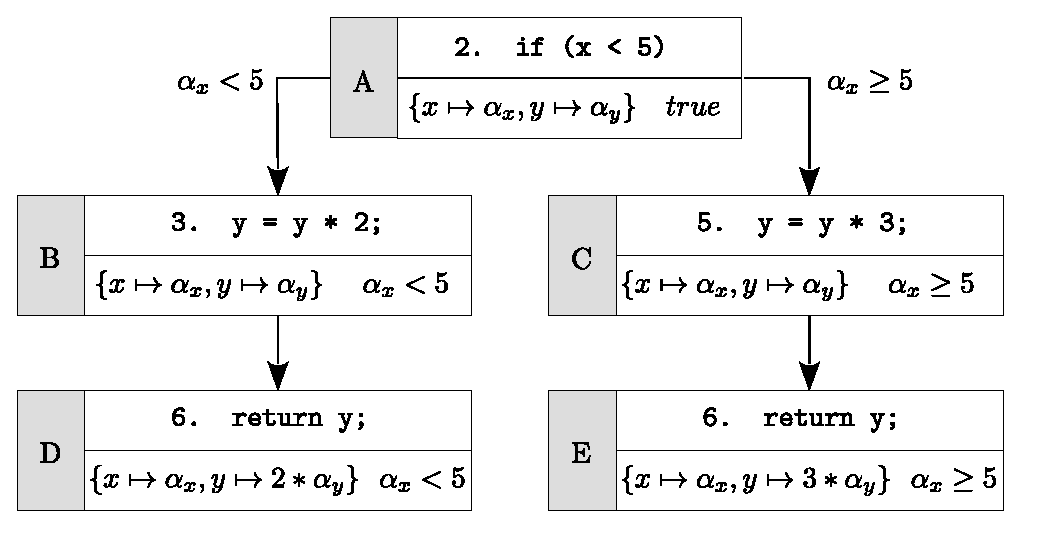
\includegraphics[width=1.05\columnwidth]{images/state-merging} 
    %\label{fig:sub1}
    \vspace{-6.5mm}
    \caption{}
  \end{subfigure}%
  \begin{subfigure}{.5\textwidth}
    \centering
    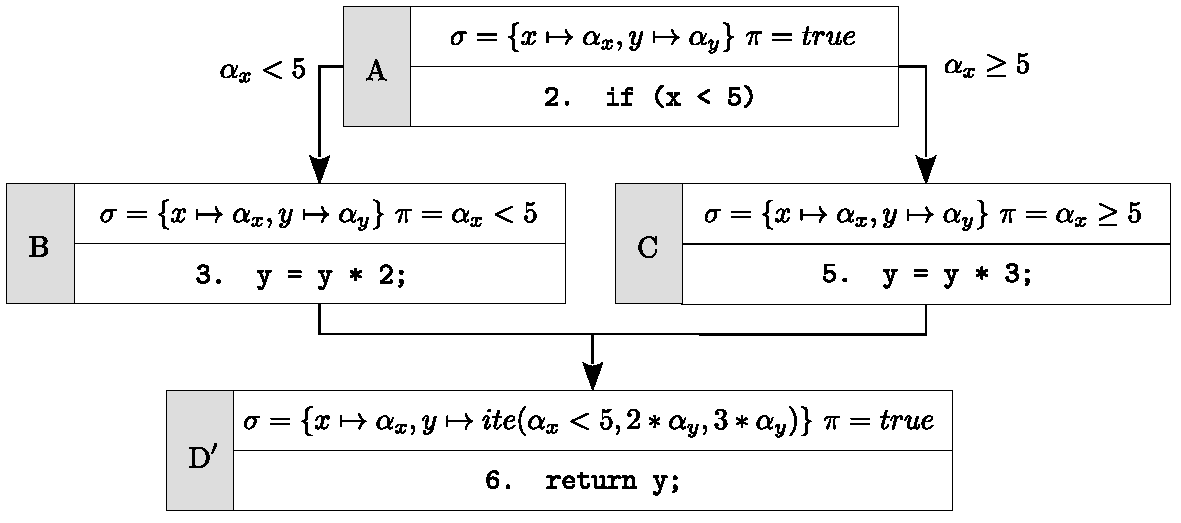
\includegraphics[width=1.05\columnwidth]{images/state-merging-2} 
    %\label{fig:sub2}
    \vspace{-4mm}
    \caption{}
  \end{subfigure}
  \vspace{-3mm}
  \caption{Symbolic execution of function \texttt{foo}: (a) without state merging; (b) with state merging.}
  \label{fig:example-state-merging}
\end{figure}

%\vspace{-4pt} % TODO
\myparagraphnoperiod{Tradeoffs: to Merge or Not to Merge?} \mytempedit{In general, it makes sense to apply state merging whenever two symbolic states, that will next evaluate the same statement, are very similar in terms of their symbolic stores (i.e., they differ only for few elements). Given two states $(stmt_1,~\sigma_1,~\pi_1)$ and $(stmt_1,~\sigma_2,~\pi_2)$, the merged state can be constructed as $(stmt,~\sigma',~\pi_1 \vee \pi_2)$, where $stmt = stmt_1 = stmt_2$, $\sigma'$ is the merged symbolic store between $\sigma_1$ and $\sigma_2$ with {\em ite}-expressions that keep track of the differences between variables, and $\pi_1 \vee \pi_2$ which is the disjunction of the path constraints coming from the two merged states. Control-flow structures such as if-else statements (e.g., as the example discussed above) or simple loops often have successors which are very similar and thus represent very good candidates for state merging.}

Early works~\cite{G-POPL07,HSS-RV09} have shown that merging techniques effectively decrease the number of paths to explore, but also put a burden on constraints solvers, which typically encounter difficulties when dealing with disjunction. Merging can also introduce new symbolic expressions in the code, for instance when merging different concrete values from a conditional assignment into a symbolic expression over the condition. \cite{KKB-PLDI12} provides an excellent discussion of the design space of state merging techniques. At the one end of the spectrum, complete separation of the paths does not perform any merge and is used in search-based symbolic execution (Section~\ref{ss:heuristics}). At the other end, static state merging combines states at control-flow join points, thus essentially representing a whole program with a single formula. Static state merging is used in whole-program verification condition generators\iffullver{, e.g.,} ~\cite{SATURN-POPL05,CALYSTO-ICSE08}), \iffullver{which typically trade precision for scalability by, for instance, unrolling loops only once.}{which usually trade precision for scalability by, e.g., unrolling loops only once.}

%At the other end, static state merging combines states at control-flow join points after all subpaths leading to a join point have been explored.

%\mynote{Function summaries}

\myparagraph{Merging Heuristics} Intermediate merging solutions adopt heuristics to identify state merges that can speed the exploration process up. Indeed, generating larger symbolic expressions and possibly extra solvers invocations can outweigh the benefit of having fewer states, leading to poorer overall performance~\cite{HSS-RV09,KKB-PLDI12}. {\em Query count estimation}~\cite{KKB-PLDI12} relies on a simple static analysis to identify how often each variable is used in branch conditions past any given point in the CFG. The estimate is used as a proxy for the number of solver queries that a given variable is likely to be part of. Two states make a good candidate for merging when their differing variables are expected to appear infrequently in later queries. {\em Veritesting}~\cite{VERITESTING-ICSE14} implements a form of merging heuristic based on a distinction between easy and hard statements. Hard statements are those that involve indirect jumps, system calls, and other operations for which precise static analyses are difficult to achieve. Static merging is performed on sequences of easy statements, %which are represented as a single path 
whose effects are captured using $ite$ expressions, 
while per-path symbolic exploration is done whenever a hard-to-analyze statement is encountered. 

%identifies sequences of statements that do not contain system calls, indirect jumps, and other statements that are difficult to reason about statically, and represents them with a single formula as in static state merging. The approach is alternated with a per-path basis symbolic exploration every time a hard-to-analyze statement is encountered. 

\myparagraph{Dynamic State Merging} Ideally, in order to maximize the opportunities for merging, a symbolic execution engine should traverse a CFG so that a combined state for a program point can be computed from its predecessors, e.g., if the graph is acyclic, by following a topological ordering. However, this would prevent search exploration strategies aiming at prioritizing more ``interesting'' states over others. \cite{KKB-PLDI12} introduces {\em dynamic state merging} to identify opportunities for merging regardless of the exploration order imposed by the search strategy.
Suppose the symbolic engine maintains a worklist of states and a bounded history of their predecessors. When the engine has to pick the next state to explore, it first checks whether there are two states $s_1$ and $s_2$ from the worklist such that they do not match for merging, but $s_1$ and a predecessor of $s_2$ do. If the expected similarity between $s_2$ and a successor of $s_1$ is also high, the algorithm attempts a merge by advancing the execution of $s_1$ for a fixed number of steps. This captures the idea that if two states are similar, then also their respective successors are likely to become similar in a few steps. If the merge fails, the algorithm lets the search heuristic pick the next state to explore.

%This is useful, for instance, for unbounded loops for which search-based symbolic execution engines would employ search strategies that prioritize exploring new code over unrolling, while static state merging would require a depth-first exploration and thus fully unroll the possibly infinitely many iterations of the loop.

% ---------------------------------------------------------------------------------------------------
\subsection{Leveraging Program Analysis and Optimization Techniques}
\label{ss:program-analysis}

A deeper understanding of a program's behavior can help a symbolic engine \mytempedit{to optimize its analysis and to focus on promising states}, e.g., by pruning uninteresting parts of the computation tree. Several classical program analysis techniques have been explored in the symbolic execution literature. \mytempedit{We now briefly discuss some prominent examples.}

% \mytempedit{In this section we explore connections with other program analysis and verification techniques.}

%is a method that, starting from a subset of a program's behavior, extracts from the program the minimal sequence of instructions that faithfully represents that behavior~\cite{Weiser84}.
\mytempedit{
\myparagraph{Program slicing} This analysis,} starting from a subset of a program's behavior, extracts from the program the minimal sequence of instructions that faithfully represents that behavior~\cite{Weiser84}. This information can help a symbolic engine in several ways: for instance, \cite{FIRMALICE-NDSS15} exploits backward program slicing to restrict symbolic exploration toward a specific target program point.

 %given a program slice related to a target program point, symbolic exploration can be restricted to paths contained in the program slice. \iffullver{We discuss an example of use in Section~\ref{ss:auth-bypass}.}{}

\mytempedit{
\myparagraph{Taint analysis}} \mytempedit{This technique~\cite{SAB-SP10}} attempts to check which variables of a program may hold values derived from potentially dangerous external sources such as user input. The analysis can be performed both statically and dynamically, with the latter yielding more accurate results. \mytempedit{In the context of symbolic execution, taint analysis can help an engine to detects which paths depend on tainted values. For instance,~\cite{MAYHEM-SP12} focuses its analysis on paths where a jump instruction is tainted and uses symbolic execution to generate an exploit.
% skip execution paths that do not depend upon tainted values, effectively reducing the exploration state space.}
%In the context of symbolic execution, taint analysis can help an engine skip execution paths that do not depend upon tainted values, effectively reducing the exploration state space~\cite{SAB-SP10}.
}

\mytempedit{
\myparagraph{Fuzzing} This software testing approach randomly mutates user-provided test inputs to cause crashes or assertion failures, possibly finding potential memory leaks.} Fuzzing can be augmented with symbolic execution to collect constraints for an input and negate them to generate new inputs. On the other hand, a symbolic executor can be augmented with fuzzing to reach deeper states in the exploration more quickly and efficiently. \mytempedit{Two notable embodiments of this idea are presented {\em hybrid concolic testing}~\cite{RK-ICSE07} and Driller~\cite{DRILLER-NDSS16}.}
%\iffullver{: we present two embodiments of this approach in Section~\ref{ss:bug-detection}.} 

%{.\mynote{CD: consider citing fuzzers formerly in the apps section}}
  %\mynote{C: crossref: dynamic test generation}
  %\footnote{\cite{DRILLER-NDSS16} classifies offline symbolic executors such as {\sc DART} and {\sc SAGE} as {\em whitebox fuzzers}.}

\mytempedit{
\myparagraph{Branch predication} This is a strategy for} mitigating misprediction penalties in pipelined executions by avoiding jumps over very small sections of code: for instance, control-flow forking constructs such as the C ternary operator can be replaced with a predicated {\tt select} instruction. \cite{CCK-EUROSYS11} reports an exponential decrease in the number of paths to explore from the adoption of this strategy when cross-checking two implementations of a program using symbolic execution. % [D] alternative formulation: ~\cite{CCK-EUROSYS11} cross-checks two implementations of a program using symbolic execution and reports an exponential decrease in the number of paths to explore from the adoption of a simple form of this strategy; 
%  \item {\em source code analysis}: \mynote{TODO/drop?} extraction of input properties (e.g., size or contents of an array);

\mytempedit{
\myparagraph{Type checking} Symbolic analysis can be effectively mixed with typed checking~\cite{KCF-PLDI10}}:  for instance, type checking can determine the return type of a function that is difficult to analyze symbolically: such information can then potentially be used by the executor to prune certain paths\footnote{Interestingly,~\cite{KCF-PLDI10} discusses also how symbolic analysis can help a type checker. For instance, a symbolic engine can provide context-sensitive properties over a variable that would rule out certain type errors, improving the precision of the type checker.}.

%\mytempedit{\myparagraph{State matching} This approach determines whether an abstract state is subsumed by another}, and can be used to analyze an under-approximation of a program's behavior. For instance, \cite{APV-SPIN06,VPP-ISSTA06} explore different heap shapes in the context of test generation for data structures, using subsumption checking to determine whether a symbolic state is being revisited. % ~\cite{XGM-ISSTA08} implements a different form of under-approximation: it looks for buffer overflows by having only a prefix of a buffer handled symbolically, and a symbolic length that may exceed the lenght of the prefix (any byte beyond the prefix is filled with concrete random data) - [D] I'm dropping this for now as we would have to call the item 'under-approximation' and change the first part of the text

\mytempedit{
\myparagraph{Classic Compiler Optimizations}
It has been also argued that program optimization techniques should be a first-class ingredient of practical implementations of symbolic execution, alongside widely accepted solutions such as search heuristics, state merging, and constraint solving optimizations~\cite{Cadar-FSE15}. In fact, program transformations can affect both the complexity of the constraints generated during path exploration and the exploration itself. For instance, precomputing the results of a function using a lookup table leads to a larger number of constraints in the path conditions due to memory accesses, while applying strength reduction for a multiplication by a constant results in a chain of addition operations that is more expensive for a constraint solver. Also, the way high-level {\tt switch} statements are compiled can significantly affect the performance of path exploration, while resorting to conditional instructions such as {\tt select} in LLVM or {\tt setcc} and {\tt cmov} in x86 can avoid expensive state forking by yielding {\em ite} expressions instead.

% D-THESIS14 superseded by DOZ-ISSRE15
%and none of them has tackled the analysis of binary programs.
While the effects of a compiler optimization can usually be predicted on the number or size of the instructions executed at run time, a similar reduction is not obvious in symbolic execution~\cite{DOZ-ISSRE15}, mostly because the constraint solver is typically used as a black-box. To the best of our knowledge, only a few works have attempted to analyze the impact of compiler optimizations on constraint generation and path exploration~\cite{WKC-HOTOS13,DOZ-ISSRE15}, leaving interesting open questions. \mynote{TODO: Move to 3.1?}Of a different flavor is the work presented in~\cite{PMZ-ISSTA17}, which explores transformations such as dynamic constant folding and optimized constraint encoding to speed up memory operations in symbolic executors based on theories of arrays (Section~\ref{ss:fully-symbolic-memory}).
}

   %%%% DROPPED PARTS
    %\item {\em compositional techniques}: caching and reusing the analysis of lower-level function in subsequent computations. The main idea is to compute function summaries. See, e.g.,~\cite{G-POPL07,G-PLDI11,MS-TR07}.
   %%%% REWRITTEN PARTS
  %\item {\em phi-node folding} is a code transformation that can be used for statically merging some paths\mynote{E: relation with state merging?}. The main idea is to replace branches with predicated select instructions. Using this technique, the number of paths that must be explored by a symbolic engine can be significantly decreased. For instance,~\cite{CCK-EUROSYS11} used an aggressive variant of phi-node folding, called {\em if-conversion}~\cite{CCF-CGO03}, that allowed them to reduce the number of paths by an exponential factor on some benchmarks.
%\item \cite{DRILLER-NDSS16} is an example of {\em symbolic-assisted fuzzing}: their technique temporarily exploits concolic execution only when a fuzzer cannot generate a valid input to explore an uncovered branch.
 % \item {\em abstraction}~\cite{C-SEFM07} is a technique that may be used for computing {\em under-approximations} or {\em over-approximations} of a program state. This approach has been exploited in prior works~\cite{APV-SPIN06,VPP-ISSTA06,XGM-ISSTA08}\mynote{check these papers}. Since some of these works reason about state subsumption, they may be connected with the incremental solving optimization discussed in Section~\ref{constraint-optimizations}.
   %\item {\em type-checking}: \cite{KCF-PLDI10} shows how symbolic analysis can be effectively mixed with type-checking analysis. For instance, type-checking analysis can help a symbolic execution engine by detecting the type of an object (e.g., the type of a value returned by a {\em hard to reason} function). Although no assumption can be made on the value of the returned type, this information may still be useful for the symbolic engine (e.g., if the type has a fixed size, some preconditions can be set, possibly pruning some paths). Similarly, symbolic analysis can help a type checker. For instance, the symbolic engine may provide context-sensitive properties over a variable that clearly rules out type errors, reducing the number of false positive given by a traditional context-insensitive type checker.
   
